% ------------------------------------------------------------------------------
% TYPO3 CMS 8.3 - What's New (English Version)
%
% @author	Patrick Lobacher <patrick@lobacher.de> and Michael Schams <schams.net>
% @license	Creative Commons BY-NC-SA 3.0
% @link		http://typo3.org/download/release-notes/whats-new/
% @language	English
% ------------------------------------------------------------------------------
% LTXE-CHAPTER-UID:		07b25346-95b1df21-a6ebe09a-49f53f41
% LTXE-CHAPTER-NAME:	Backend User Interface
% ------------------------------------------------------------------------------

\section{Interfaccia utente Backend}
\begin{frame}[fragile]
	\frametitle{Interfaccia utente Backend}

	\begin{center}\huge{Capitolo 1:}\end{center}
	\begin{center}\huge{\color{typo3darkgrey}\textbf{Interfaccia utente Backend}}\end{center}

\end{frame}

% ------------------------------------------------------------------------------
% LTXE-SLIDE-START
% LTXE-SLIDE-UID:		abbc1485-24b27795-13403ff0-5133ed1c
% LTXE-SLIDE-ORIGIN:	a5b4032f-741b8eea-643674fb-4dc14f50 English
% LTXE-SLIDE-TITLE:		!Feature: #20446 - Clear cache entry in context menu
% LTXE-SLIDE-REFERENCE:	!Feature-20446-ClearCacheEntryInContextMenu.rst
% ------------------------------------------------------------------------------
\begin{frame}[fragile]
	\frametitle{Interfaccia utente Backend}
	\framesubtitle{"Clear Cache" nel menu contestuale}

	Una nuova voce è stata aggiunta nel menu dell'albero delle pagine. L'oggetto è posizionato dentro "Page Actions"
	e permette di cancellare la cache della pagina selezionata.

	\begin{figure}
		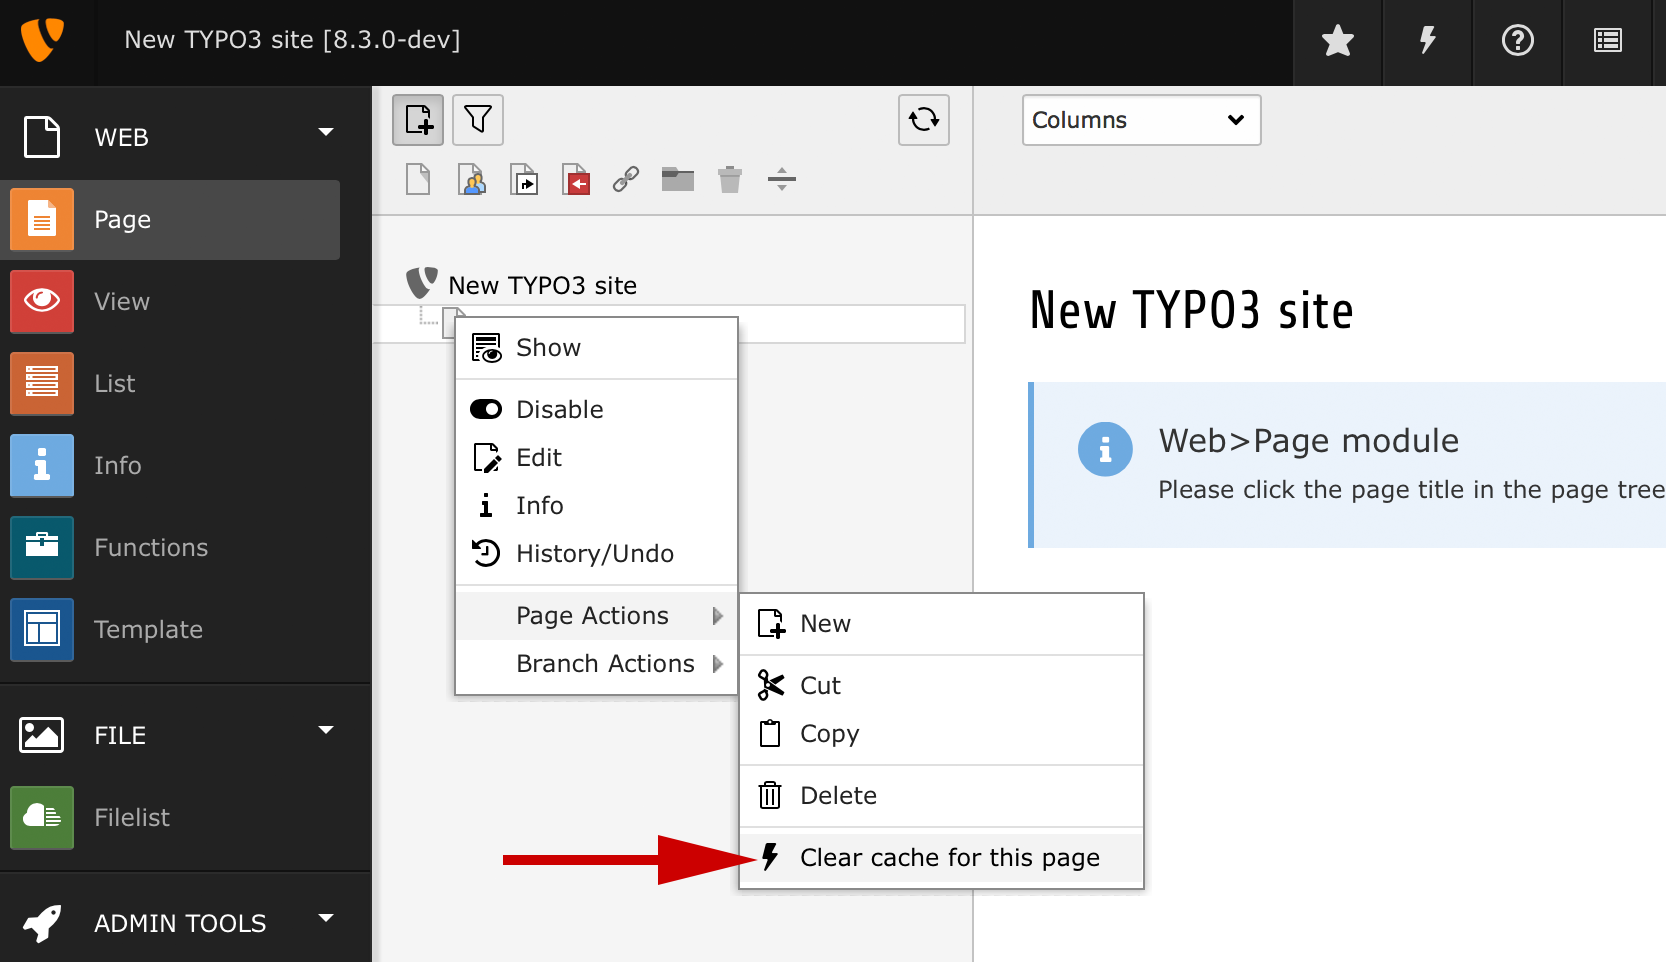
\includegraphics[width=0.70\linewidth]{BackendUserInterface/20446.png}
	\end{figure}

\end{frame}

% ------------------------------------------------------------------------------
% LTXE-SLIDE-START
% LTXE-SLIDE-UID:		53cee076-4f6b8f36-d9276ff7-246e8eb7
% LTXE-SLIDE-ORIGIN:	5b0090eb-13043388-8c4dee34-6cac1521 English
% LTXE-SLIDE-TITLE:		!Feature: #76072 - Ogg, flac and opus support
% LTXE-SLIDE-REFERENCE:	!Feature-76072-OggFlacAndOpusSupport.rst
% ------------------------------------------------------------------------------
\begin{frame}[fragile]
	\frametitle{Interfaccia utente Backend}
	\framesubtitle{Compatibilità Ogg, Flac e Opus}

	La compatibilità con i seguenti formati aperti è stata aggiunta al campo media:
	\texttt{ogg}, \texttt{flac} e \texttt{opus}

	\begin{figure}
		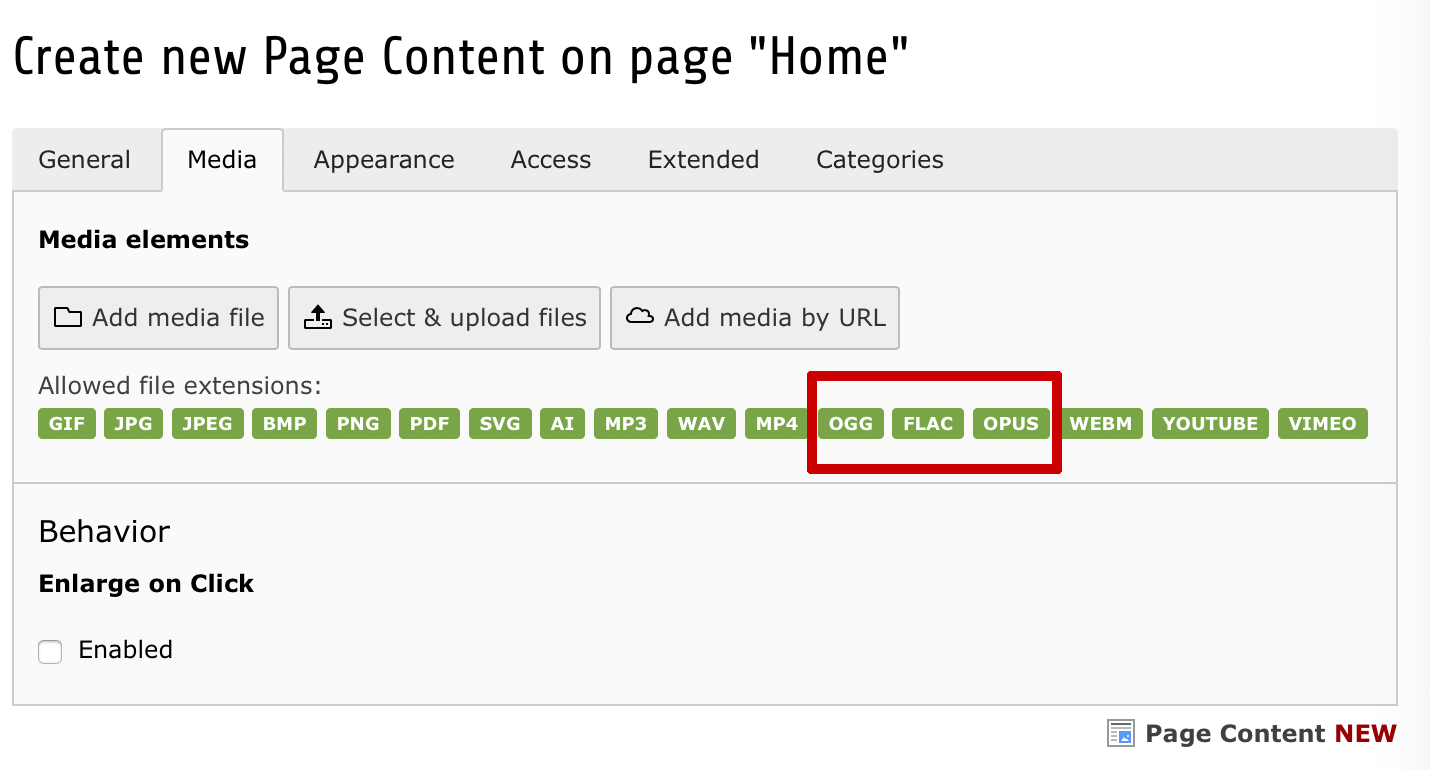
\includegraphics[width=0.70\linewidth]{BackendUserInterface/76072.png}
	\end{figure}

\end{frame}


